\section{Regra da Cadeia em Fun\c{c}\~oes de 2 Vari\'aveis} 
Dada a fun\c{c}\~ao
\begin{equation*}
    f(x,y) = e^{x(\xi, \eta)} + e^{\sin(x(\xi, \eta) y(\xi, \eta)^3)}
\end{equation*}
calcule o gradiente relativo \`as coordenadas param\'etricas $\xi$ e $\eta$, sobre a superf\'icie parametrizada dada por:
\begin{equation*}
    \begin{cases}
        x(\xi, \eta) = \cos(\xi^2) + \sin(\eta + 1) + 5\xi \\
        y(\xi, \eta) = \sin(\xi^3) + \cos(\eta^2) + 7\eta
    \end{cases}.
\end{equation*}

\subsection{Solu\c{c}\~ao}
O exerc\'icio 3 foi feito utilizando o \textit{software} \texttt{Mathematica} e o c\'odigo utilizado pode ser encontrado no Ap\^endice \ref{sec:github}. 

O gradiente de $f$ em rela\c{c}\~ao \`as coordenadas param\'etricas $\xi$ e $\eta$ \'e dado pela regra da cadeia, expressa pela Eq. \eqref{eq:gradfxy}
\begin{equation}
    \label{eq:gradfxy}   
    \grad{f} = \begin{bmatrix}
        \frac{\partial f}{\partial \xi} \\
        \frac{\partial f}{\partial \eta}
    \end{bmatrix} = 
    \begin{bmatrix}
        \frac{\partial f}{\partial x} \frac{\partial x}{\partial \xi} + \frac{\partial f}{\partial y} \frac{\partial y}{\partial \xi} \\
        \frac{\partial f}{\partial x} \frac{\partial x}{\partial \eta} + \frac{\partial f}{\partial y} \frac{\partial y}{\partial \eta}
    \end{bmatrix}
\end{equation}
logo, basta evaluar as derivadas parciais $\frac{\partial f}{\partial x}$, $\frac{\partial f}{\partial y}$, $\frac{\partial x}{\partial \xi}$, $\frac{\partial x}{\partial \eta}$, $\frac{\partial y}{\partial \xi}$ e $\frac{\partial y}{\partial \eta}$  e depois substituir na Eq. \eqref{eq:gradfxy}.

Utilizando o \texttt{Mathematica} obt\'em-se que: 
\begin{equation*}
    \frac{\partial f}{\partial x} = e^x + y^3 e^{\sin \left(x
    y^3\right)} \cos \left(x
    y^3\right)
\end{equation*}
\begin{equation*}
    \frac{\partial f}{\partial y} = 3 y^2 e^{\sin \left(x
    y^3\right)} \cos \left(x
    y^3\right)
\end{equation*}
\begin{equation*}
    \frac{\partial x}{\partial \xi} = -2 \xi \sin \left(\xi^2\right) + 5
\end{equation*}
\begin{equation*}
    \frac{\partial x}{\partial \eta} = \cos \left(\eta + 1\right)
\end{equation*}
\begin{equation*}
    \frac{\partial y}{\partial \xi} = 3 \xi^2 \cos \left(\xi^3\right)
\end{equation*}
\begin{equation*}
    \frac{\partial y}{\partial \eta} = -2 \eta \sin \left(\eta^2\right) + 7.
\end{equation*}

Dados a complexidade e o tamanho das fun\c{c}\~oes que comp\~oem o gradiente, optou-se por apresentar um trecho do c\'odigo utilizado em que o gradiente \'e calculado. As figuras \ref{fig:dfdxi} e \ref{fig:dfdeta} mostram o c\'alculo das derivadas parciais $\frac{\partial f}{\partial \xi}$ e $\frac{\partial f}{\partial \eta}$, respectivamente.

\begin{figure}[H]
    \centering
    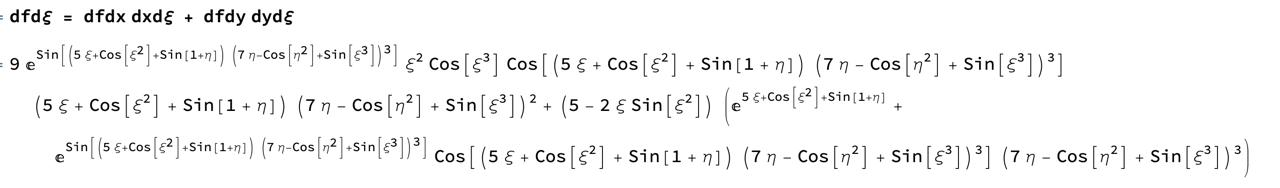
\includegraphics[scale=.38]{Figures/Ex3dfdxi.jpeg}
    \caption{C\'alculo da derivada parcial $\frac{\partial f}{\partial \xi}$.}
    \label{fig:dfdxi}
\end{figure}

\begin{figure}[H]
    \centering
    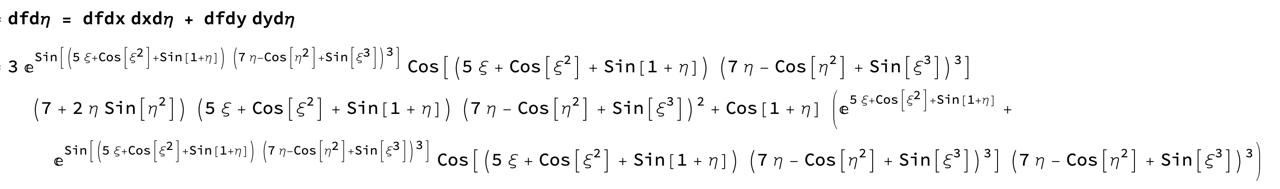
\includegraphics[scale=.38]{Figures/Ex3dfdeta.jpeg}
    \caption{C\'alculo da derivada parcial $\frac{\partial f}{\partial \eta}$.}
    \label{fig:dfdeta}
\end{figure}

Apresenta-se tamb\'em a compara\c{c}\~ao entre os resultados obtidos pela regra da cadeia programada e pelas fun\c{c}\~oes nativas do \texttt{Mathematica}

\begin{figure}[H]
    \centering
    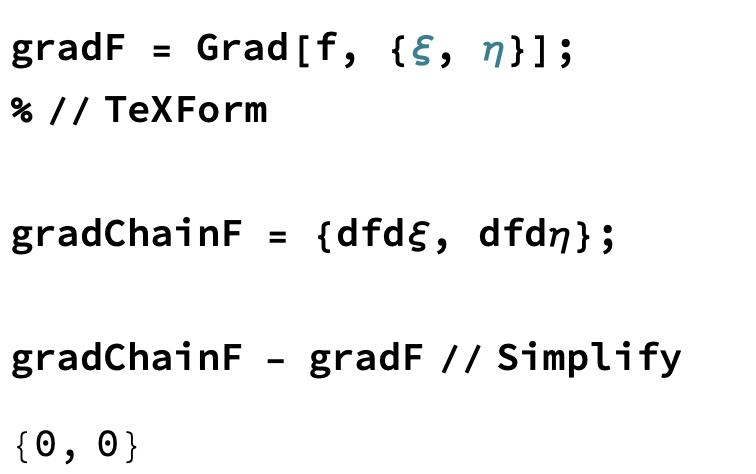
\includegraphics[scale=.22]{Figures/Ex3Comparison.jpeg}
    \caption{Compara\c{c}\~ao entre gradientes: $gradF$ - \texttt{Mathematica} e $gradChainF$ - Regra da Cadeia.}
    \label{fig:gradf}
\end{figure}

Como mostrado pela Fig. \ref{fig:gradf}, os resultados alcan\c{c}ados pela regra da cadeia e pelo \texttt{Mathematica} s\~ao iguais, j\'a que a diferen\c{c}a entre os gradientes \'e nula. Tal fato confirma que a implementa\c{c}\~ao da regra da cadeia est\'a correta. Por fim, plota-se os gr\'aficos do gradiente de $f(x(\xi, \eta), y(\xi, \eta))$ na Fig. \ref{fig:gradfplot}.

\begin{figure}[H]
    \centering
    \subfloat[\label{fig:plotGradf}]{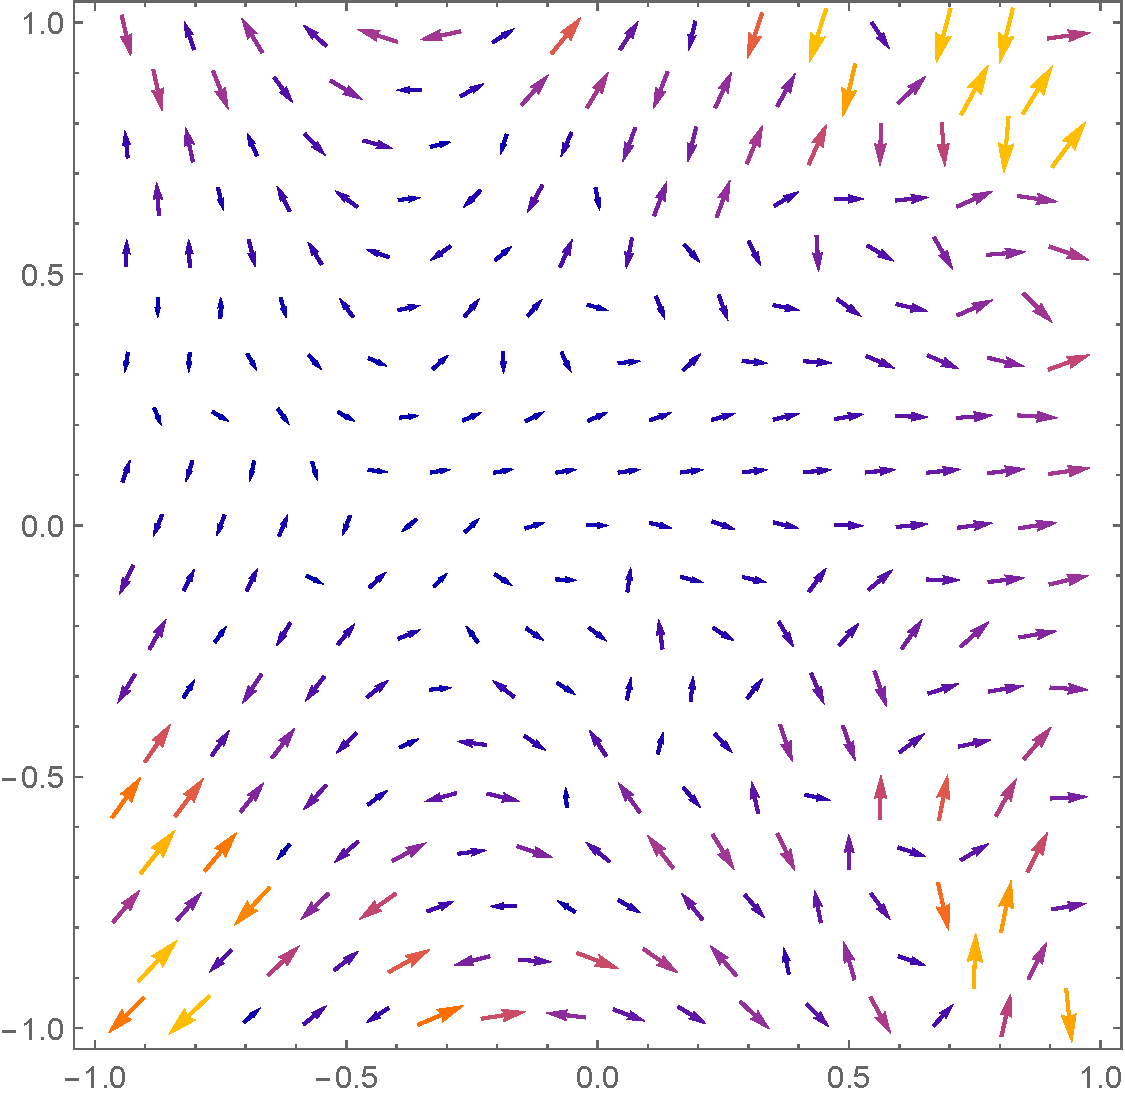
\includegraphics[width=0.49\textwidth]{Ex3GradF.pdf}}\hfill
    \subfloat[\label{fig:contourF}]{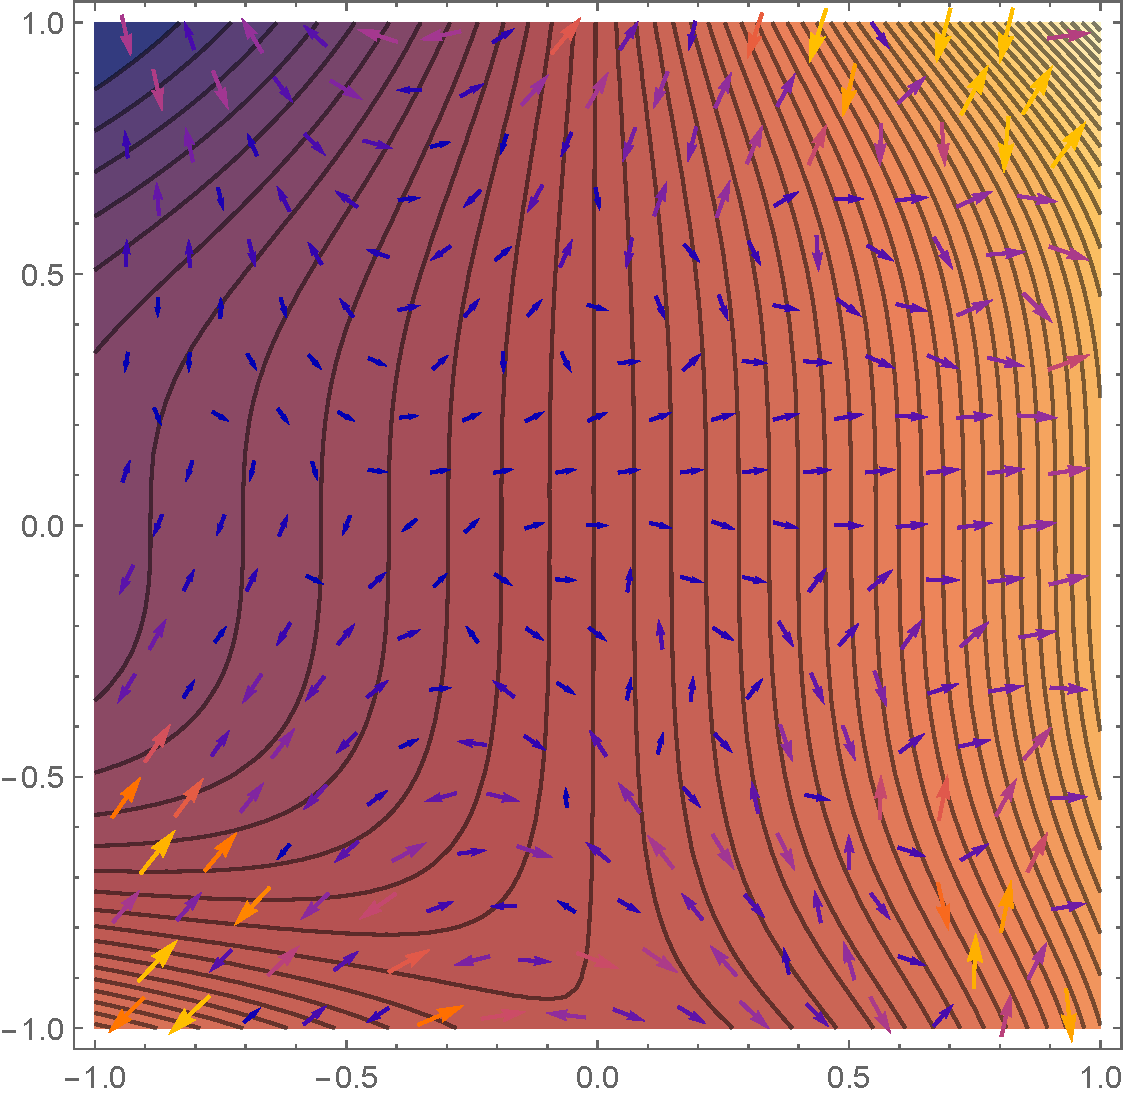
\includegraphics[width=0.49\textwidth]{Ex3ContourF.pdf}}
    \caption{Resultados: a) gradiente de $f$. b) Contorno de $f$.}
    \label{fig:gradfplot}
\end{figure}